\documentclass[a4paper,openright,12pt]{book}
\usepackage[spanish,  es-tabla]{babel} 
\usepackage[latin1]{inputenc}
\usepackage{graphicx}	
\usepackage{multirow, array}
\usepackage{longtable}
\usepackage{graphicx}
\usepackage{colortbl}
\usepackage{listings}

\begin{document}

\begin{titlepage}

\begin{center}
\vspace*{-1in}
\begin{figure}[htb]
\begin{center}

\includegraphics[width=8cm]{ciencias2}
\end{center}
\end{figure}

FACULTAD DE CIENCI\\
\vspace*{0.15in}
DEPARTAMENTO DE MATEMATICAS\\
\vspace*{0.6in}
\begin{large}
EXPERIENCIA PROFESIONAL\\
\end{large}
\vspace*{0.2in}
\begin{Large}
\textbf{Implementaci\'on de un nuevo modelo de consulta de informaci\'on y reestructura de arquitectura de datos} \\
\end{Large}
\vspace*{0.3in}
\begin{large}
Trabajo por experiencia profesional presentado por Erick Celso Zavaleta Gonz\'alez para obtener el grado de Licenciado \\
\end{large}
\vspace*{0.3in}
\rule{80mm}{0.1mm}\\
\vspace*{0.1in}
\begin{large}
Supervisados por: \\
Dr. Canek Pel\'aez Val\'es \\
\end{large}
\end{center}

\end{titlepage}

\newpage
$\ $
\thispagestyle{empty} % para que no se numere esta pagina

\chapter*{}
\pagenumbering{Roman} % para comenzar la numeracion de paginas en numeros romanos
\begin{flushright}
\textit{Dedicado a... \\}
\end{flushright}


\chapter*{Agradecimientos} % si no queremos que a�ada la palabra "Capitulo"
\addcontentsline{toc}{chapter}{Agradecimientos} % si queremos que aparezca en el �ndice
\markboth{AGRADECIMIENTOS}{AGRADECIMIENTOS} % encabezado 
 
�Muchas gracias a todos!

\tableofcontents % indice de contenidos

\cleardoublepage
\addcontentsline{toc}{chapter}{Lista de figuras} % para que aparezca en el indice de contenidos
\listoffigures % indice de figuras

\cleardoublepage
\addcontentsline{toc}{chapter}{Lista de tablas} % para que aparezca en el indice de contenidos
\listoftables % indice de tablas

\chapter*{Marco Te\'orico} \label{cap.mteorico}% si no queremos que a�ada la palabra "Capitulo"
\pagenumbering{arabic}
\addcontentsline{toc}{section}{Marco Te\'orico} % si queremos que aparezca en el �ndice
\markboth{Marco Te\'orico}{Marco Te\'orico} % encabezado

El marco te\'orico del proyecto se basa en laarquitecura de datos, que en tecnolog\'ia de la informaci\'on se compone de los modelos, pol\'iticas, reglas y/o est\'andares que determinan qu\'e datos se recolectan y c\'omo se guardan, ordenan, integran y usan en los sistemas de datos de una instituci\'on.

Hablar de datos es entrar en un mundo complejo donde existen diferentes perspectivas de datos, dependiendo del uso que se les quiera dar o de las personas que lo utilizan. Cada grupo de personas tiene su propia perspectiva sobre el manejo de datos: manejo de grandes vol\'umenes, acceso al detalle de los datos de manera instant\'anea, manejo de la integridad, datos de acceso exclusivo, etc. La arquitectura de datos nos ayuda a que estos diferentes tipos de datos y diferentes necesidades puedan coexistir de una forma conjunta de acuerdo a las necesidades de cada \'area o empresa. 

Actualmente no existe ning\'un secreto para el manejo de datos y su respectiva arquitectura; en ambos casos, es importante entender los datos en t\'erminos de su infraestructura; es decir, se requiere conocer la infraestructura que rodea a los datos para llevar a cabo un uso adecuado de los mismos.

As\'i mismo, es importante saber que dentro de cualquier empresa u organizaci\'on se pueden encontrar diferentes tipos de datos: estructurados y no estructurados. Los primeros son datos predecibles y que normalmente son manejados en una base de datos (SMBD): registros, atributos, llaves, \'indices, etc. Por su parte, los datos no estructurados no son predecibles y, como su nombre lo indica, no tienen una estructura bien definida, usualmente son de dificil acceso y generalmente se requiere una b\'usqueda m\'as profunda para hacer consultas; por ejemplo, una cadena de car\'acteres en un texto libre. 

Todos estos conceptos ser\'an detallados y aplicados en los cap\'itulos del proyecto presentado.


\chapter*{Objetivo y Justificaci\'on} \label{cap.objetivo}% si no queremos que a�ada la palabra "Capitulo"
\addcontentsline{toc}{section}{Objetivo y Justificaci\'on} % si queremos que aparezca en el �ndice
\markboth{Objetivo y Justificaci\'on}{Objetivo y Justificaci\'on} % encabezado

El proyecto que se presenta fue la implementaci\'on y reestructura de la infraestructura de base de datos, as\'i como los cambios en procesos y arquitectura de datos de una instituci\'on financiera que por razones de acuerdos de confidencialidad no puedo mencionar su nombre. Dentro de las actividades que realic\'e se encuentra un an\'alisis del software a utilizar, as\'i como la definici\'on y desarrollo de programas para convertir los datos de diferentes bases de datos y plataformas hacia un repositorio de datos \'unico que ayud\'o a eficientar los tiempos de respuesta y las consultas realizadas.

Las bases en desarrollo de software, bases de datos, estructuras de datos, lenguajes de programaci\'on y, por encima de todo, an\'alisis y soluci\'on de problemas que obtuve dentro de la carrera de Ciencias de la Computaci\'on, me ayudar\'on a que dicho proyecto se realizara de manera \'exitosa.  



\chapter{An\'alisis de requerimientos} \label{cap.analisis}% si no queremos que a�ada la palabra "Capitulo"
\addcontentsline{toc}{section}{An\'alisis de requerimientos} % si queremos que aparezca en el �ndice
\markboth{An\'alisis de requerimientos}{An\'alisis de requerimientos} % encabezado

\section{Proceso de selecci\'on de software}
Parte importante para llegar a la soluci\'on propuesta fue la selecci\'on del software en el cual se desarroll\'o el nuevo proceso ETL \footnote{Extracci\'on, Transformaci\'on y Carga (Load en Ingl\'es)}. La selecci\'on de software requiri\'o de varios pasos previos a la toma de la decisi\'on. El proceso de selecci\'on de software de acuerdo a la metodolog\'ia de Accenture fue la siguiente:


\begin{enumerate}
\item Establecer los requerimientos de negocio
\item Establecer los requerimientos de evaluaci\'on de las herramientas de ETL
\item Generar una lista larga de proveedores
\item Generar una lista corta (generalmente 3 o 4 prveedores) de candidatos
\item Realizar un RFP (Request For Approval) para evaluar a los candidatos de manera individual y detallada
\item Realizar la recomendaci\'on final del producto. 
\end{enumerate}

Este proceso se datalla en la siguiente figura:
\begin{figure}[htb]
  \begin{center}
    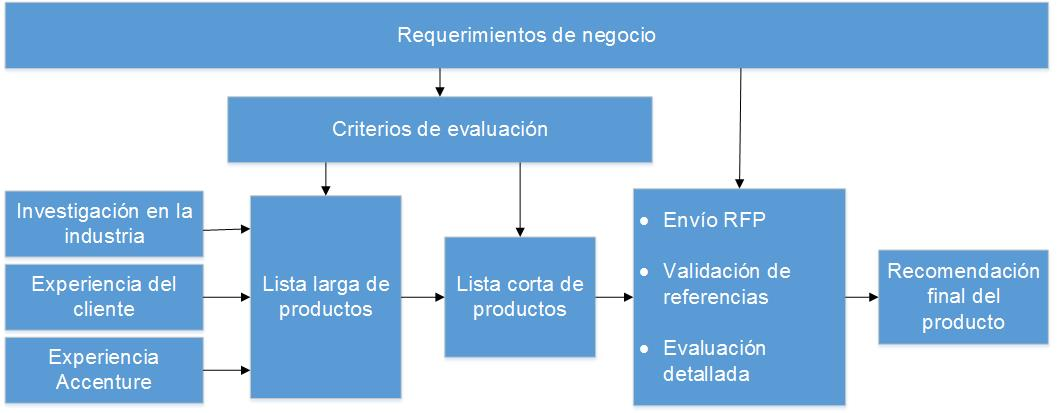
\includegraphics[width=12cm, height=3cm, scale=0.5]{Proceso_seleccion_software.jpg}
        \caption{Proceso de selecci\'on de software}
    \label{fig:proceso}
  \end{center}
\end{figure}

En las siguientes secciones se definir\'an cada uno de los pasos del proceso seguidos.

\subsection{Requerimientos funcionales}

Con base en las reuniones realizadas con el \'area de desarrollo de sistemas de la instituci\'on financiera se identificaron una serie de requerimientos funcionales detallados a continuaci\'on. 

\begin{itemize}
\item Se requer\'ia una conexi\'on a correo electr\'onico mediante le protocolo SMTP para env\'io de informes de termino de procesos o de error en los mismos.
\item Tener un log de procesos que tuviera la informaci\'on de cada uno de los procesos de extracc\'on/carga  (inicio, fin, estatus de termino, errores (en cso de haberlos)).
\item La herramienta deb\'ia de tener la capacidad de contar con un esquema de limpieza de datos que permitiera identificar y corregir los errores en nombres, direcciones, RFC's, n\'umeros de tel\'efono, y algunos otros datos relevantes para la instituci\'on financiera.
\item Permitir invocar a la herramienta ETL desde otras aplicaciones tales como PeopleSoft, aplicaciones desarrolladas en Java y .NET.
\item Permitir control y detalle de los errores presentados en los procesos o en cada uno de los componentes del flujo de datos. El control se llevaría a cabo mediante el env\'io, por parte del ETL, de errores a tablas log o archivos de texto en dode se pudieran identificar de una manera sencilla, los errores presentados.
\item Contar con un esquema de datos redundante, como puede ser un cluster, bases de datos replicadas, balanceo de cargas con tolerancia a fallos, etc.
\item Contar con un esquema de control de versiones que soporte el trabajo de multiples usuarios al mismo tiempo.
\item La herramienta deb\'ia tener la capacidad para entregar diferentes archivos a los sistemas destino (archivos de texto, tablas en base de datos, XML, PDF, Excel).
\item Contar con un esquema de seguridad basado en roles y jerarqu\'ias de usuario que permitieran a los usuarios acceder a datos espec\'ificos de la base de datos de acuerdo a su rol.
\item Contar con pantallas de configuraci\'on que permitieran a los administradores de la herramienta tener un mayor control sobre los procesos y los usuarios. As\'i mismo, que fuera una herramienta visualmente f\'acil de usar.
\item Permitir a la nueva herramienta la convivencia con las tecnolog\'ias con las que contaba la instituci\'on financiera (Windows 2003, SQL Server 2005, Oracle, DB2, AS400, Windows Vista y Mainframes)
\item Contar con una herramienta de f\'acil manejo de metadatos. 
\item Contar con un ambiente de dise\~no y desarrollo 100\% visual que permitiera a los desarrolladores implementar las soluciones de extracci\'on y carga de una manera sencilla.
\item Permitir la operaci\'on y administraci\'on de la herramienta de una forma remota.
\item Generar componentes reutilizables entre aplicaciones y entre procesos.
\item La herramienta deb\'ia permitir a los usuarios, la creaci\'on de funciones personalizadas que cumplieran con los est\'andares de la empresa y que no fueran parte de las configuraciones predefinidas de la herramienta.
\item Capacidad para calendarizar procesos; es decir, la herramienta deber\'ia ser capaz de ejecutar los procesos de forma autom\'atica a la hora y d\'ia especificados.
\item Soportar modelos de miner\'ia de datos que ayudar\'ian  a la instituci\'on financiera a realizar un ana\'alisis de sus datos y poder definir estrategias de mercado para los diferentes productos que ofec\'ian.
\item Capacidades de soporte para DataWarehouse y Business Intelligence, este requerimiento era para cumplir con el plan estrat\'egico de la instituci\'on. 
\item Capacidad de la herramienta para plublicar procesos como Web Services a fin de poder acceder a ellos de manera remota o ejecutarlos a trav\'es de un portal con los permisos correspondientes. 
\item Capacidades de detecci\'on y correci\'on de errores en los procesos, mediante un proceso de depuraci\'on (Debugging) que ser\'ia ejecutado paso a paso.
\item Como un requerimiento b\'asico, la herramienta deber\'ia de almacenar la informaci\'on extra\'ida en una sola fuente de datos, para la soluci\'on propuesta fue una base de datos de paso llamada base de datos stage.
\item Explotaci\'on de la informaci\'on de una base centralizada para realizar reportes.
\item Consulta de datos hist\'oricos, en especial de transacciones, para poder ser explotados desde otro ambiente o aplicaci\'on existente en la instituci\'on financiera.
\item La herramienta deber\'ia de ser capaz de obtener solamente la informaci\'on que tuvo cambios entre los diferentes periodos de extracci\'on, ayudando al rendimiento del proceso y extrayendo una cantidad menor de datos.
\end{itemize} 

\subsection{Requerimientos t\'ecnicos}

Por su parte los requerimientos t\'ecnicos solicitados por la instituci\'on para seleccionar la herramienta fueron los siguientes:

\begin{itemize}
\item Mejorar el rendimiento de la extracci\'on de datos de 90 minutos a 45 minutos (tiempo tentativo) con una cantidad de 6 millones de registros
\item Mejorar el tiempo de transformaci\'on de datos utilizando componentes para limpieza y calidad de los datos.
\item Mejorar el rendimiento de la herramienta cuando el volumen de datos exceda los 100 millones de registros.
\item Que la arquitectura de la herramienta fuera compatible con la arquitectura de la instituci\'on y la futura que se plante\'o en el presente proyecto.
\item La herramienta deb\'ia ser capaz de poder integrarse son los sistemas de la instituci\'on (PeopleSoft, Core bancario, systema de reportes, sistema de recursos humanos, pagos a terceros, etc.)
\item La herramienta deb\'ia ser capaz de ejecutarse en diferentes paltaformas (Windows, Linux, Unix, Mainframes).
\item Conectividad con los istemas fuentes (ODBC, OLAP, LDAP) y con diferentes sistemas manejadores de bases de datos como Oracle, DB2, SQL Server, Informix, Sybase, Teradata.
\item Capacidad para crear funciones y  m\'etodos desde cualquier lenguaje de programaci\'on estructurado y que pudiera ser ejecutado desde la herramienta ETL.
\end{itemize}

Aunque el gobierno de datos no era parte del alcance del proyecto, pero si de la estrategia de crecimiento de la instituci\'on, la herramienta deber\'ia de soportar esta funcionalidad.

\subsection{Requerimientos de limpieza de datos}
Como parte de la definici\'on de requerimientos funcionales que deb\'ia cumplir la herramienta, existe una secci\'on que ten\'ia que ver con la calidad y limpieza de datos; estos requerimientos solicitados por parte del \'area de tecnolo\'ia fueron los siguientes: 

Se requer\'ia que el proceso ETL realizara la limpieza de datos de los campos descritos a continuaci\'on: 
\begin{itemize}
\item RFC. Se requer\'ia que el RFC se encontrara estandarizado y cumplieran con los requerimientos establecidos por el bur\'o de cr\'edito
\item Nombres de socios. Se requer\'ia que los nombres de socios no tuvieran caracteres especiales como puntos, comas, retornos de carro, par\'entesis, corchetes, porcentaje, comillas y caracteres de 16 bits.
\item Fechas de morosidad. Se solicit\'o que las fechas para el c\'alculo de la morosidad se encontraran en un formato de fecha correcto yyyymmdd y que no se permitieran valores nulos o negativos para este tipo de dato.
\item Direcciones de socios. Fue requerido que las direcciones de los socios tuvieran una nomenclatura est\'andar para nombres de calles, colonias
\item Ciudades/Municipios. Los c\'odigos y nombres de ciudades y municipios deb\'ian de contar con un est\'andar y estos deberian de estar corregidos de a cuerdo a la informaci\'on proporcionada por SEPOMEX.
\item Tel\'efonos. Los tel\'efonos de los clientes deb\'ian contar con la clave lada y todos ten\'ian que ser de 10 d\'igitos para n\'umeros fijos y de 13 d\'igitos para n\'umeros celulares
\item Los n\'umeros telef\'onicos no deber\'ian de tener guiones o caracteres especiales.
\end{itemize}

Como parte de la estandarizaci\'on de direcciones era requerido que todos los c\'odigos postales se encontraran conforme a la lista proporcionada por SEPOMEX y todos deber\'ian de ser de 5 d\'igitos.

\section{Criterios de evaluaci\'on}
Como mencionamos al inicio del documento, parte importante de la selecci\'on de sofware fue la definici\'on de los criterios de evaluaci\'on de la herramienta ETL a utilizar como parte del proyecto. Dichos criterios nos ayudaron a realizar una evaluaci\'on objetiva de las diferentes herramientas y tener un panorama general de los productos que cumpl\'ian con las caracteristicas y necesidades de la instituci\'on financiera. Tomando como base esas necesidades y la experiencia de Accenture se definieron los criterios de selecci\'on de software.

Los criterios se agruparon en conceptos genericos que describen la funcionalidad de cada \'area. Estos criterios se listan a continuaci\'on:

\begin{enumerate}
\item \textit{Capacidades del servicio}.
\item \textit{Opciones de integraci\'on}
\item \textit{Ambiente de la herramienta}
\item \textit{Soporte y capacitaci\'on}
\item \textit{T\'ecnicas adicionales de integraci\'on de datos}
\item \textit{Manejo de la informaci\'on}
\item \textit{Estrategias del producto}
\item \textit{Estrategias corporativas}
\item \textit{Costos}
\item \textit{Convenios con otros proveedores}
\item \textit{Finanzas de la compa\~nia}
\end{enumerate} 

\subsection{Lista de proveedores}
Una vez que se definieron los criterios de evaluaci\'on y se realiz\'o el an\'alisis de requerimientos con el equipo de la instituci\'on financiera, el siguiente paso fue dar una lista larga de proveedores candidatos para ser evaluados y que en ese momento eran las mejores opciones dentro del mercado. La lista conten\'ia a 6 proveedores de software: Oracle (Oracle Warehouse Builder), Inform\'atica (Power Center), IBM (Infosphere Information Server), Microsoft (Integration Services (SSIS), SAP (SAP-Business Objects), SAS Institute (SAS).


\subsection{Evaluaci\'on de proveedores} 
Con la lista larga de proveedores definida, la siguiente tarea que se llev\'o a cabo fue la evaluaci\'on de cada uno de los proveedores con el fin de establecer un grupo reducido de candidatos que representar\'ia la lista final de selecci\'on de la herramienta ETL a utilizar dentro del proyecto. De acuerdo a las necesidades de la Instituci\'on financiera se definieron los siguientes porcentajes para los criterios de evaluaci\'on


\begin{table}[htbp]
\begin{center}
\begin{tabular}{|p{6cm}|>{\centering\arraybackslash}m{3cm}|c|}
\hline
Criterio & Porcentaje de evaluaci\'on & Prioridad\\
\hline 
Capacidades del servicio & 14\% & 1 \\
\hline
Manejo de la informaci\'on & 14\% & 2\\ 
\hline
Opciones de integraci\'on & 11\% & 3\\ 
\hline
Ambiente de la herramienta & 11\% & 4\\
\hline
Costos & 11\% & 5\\
\hline
Soporte y capacitaci\'on & 9\% & 6\\
\hline
Estrategias del producto & 6\% & 7\\
\hline
Convenios con otros proveedores & 6\% & 8\\
\hline
T\'ecnicas adicionales de integraci\'on de datos & 6\% & 9\\
\hline
Estrategias corporativas & 6\% & 10\\
\hline
Finanzas de la compa\~nia proveedora & 6\% & 11\\
\hline
\end{tabular}
\caption{Porcentajes y prioridades de evaluaci\'on.}
\label{tabla:criterios}
\end{center}
\end{table}

La prioridad de cada uno de los criterios de evaluaci\'on se realiz\'o con base en las necesidades de la instituci\'on y basados tambi\'en en la funcionalidad de cada uno de ellos. 

Con toda la informaci\'on que se recolect\'o, realic\'e un an\'alisis de cada proveedor y su herramientas presentadas, as\'i como sus factores diferenciales y las caracter\'isticas principales soportadas. Esta evaluaci\'on se presenta en la siguiente tabla con los resultados finales:


\begin{table}[htbp]
\begin{center}
\scalebox{0.75}[0.65]{
\begin{tabular}{|p{5.5cm}|>{\centering\arraybackslash}m{1.7cm}|c|c|c|c|c|c|}
\hline
& & \rotatebox{90}{Microsoft SSIS} & \rotatebox{90}{Oracle OWB} & \rotatebox{90}{Inform\'atica Power center} & \rotatebox{90}{IBM IIS} & \rotatebox{90}{SAP\-Business Objects} & \rotatebox{90}{SAS} \\
\hline
&Porcentaje&&&&&&\\
\hline
\rowcolor[gray]{0.9}\textbf{Capacidades del servicio} & \textbf{14.29\%} & \textbf{3} & \textbf{3.5} & \textbf{4.5} & \textbf{4} & \textbf{3.75} & \textbf{4} \\
\hline
\rightline{Escalabilidad y rendimiento} & & 4 & 4 & 5 & 5 & 4 & 4 \\
\hline
\hspace{0.5cm}Alta disponibilidad & & 4 & 3 & 4 & 4 & 4 & 3\\
\hline
\rightline{Seguridad} & & 3 & 4 & 5 & 3 & 4 & 5\\
\hline
\hspace{0.5cm}Plataformas de ejecuci\'on soportadas & & 1 & 3 & 4 & 4 & 3 & 4\\
\hline
\rowcolor[gray]{0.9}\textbf{Opciones de integraci\'on} & \textbf{11.43\%} & \textbf{3} & \textbf{3} & \textbf{4} & \textbf{4} & \textbf{3.4} & \textbf{3.6}\\
\hline
Conectividad con sistemas fuente & & 4 & 3 & 5 & 5 & 5 & 5\\
\hline
Conectividad para la carga & & 4 & 3 & 5 & 5 & 5 & 5\\
\hline
Servicios Web & & 4 & 4 & 5 & 5 & 3 & 3\\
\hline
Conexi\'on a correo electr\'onico & & 1 & 1 & 1 & 1 & 0 & 1\\
\hline
Reusabilidad & & 2 & 4 & 4 & 4 & 4 & 4\\
\hline
\rowcolor[gray]{0.9}\textbf{Ambientes de la herramienta} & \textbf{11.43\%} & \textbf{3.2} & \textbf{4} & \textbf{4.4} & \textbf{4.2} & \textbf{4.4} & \textbf{3.6} \\
\hline
Visualizaci\'on del ambiente de dise\~no y desarrollo & & 4 & 4 & 4 & 4 & 4 & 4\\
\hline
Manejo de errores & & 4 & 4 & 5 & 4 & 5 & 4\\
\hline
Ambiente de colaboraci\'on & & 2 & 4 & 4 & 4 & 4 & 3\\
\hline
Manejo y modelado de datos y metadatos & & 2 & 4 & 4 & 4 & 4 & 4 \\
\hline 
Administraci\'on & & 4 & 4 & 5 & 5 & 5 & 3\\
\hline
\rowcolor[gray]{0.9}\textbf{Soporte y capacitaci\'on} & \textbf{8.57\%} & \textbf{4.25} & \textbf{4.75} & \textbf{4.25} & \textbf{4.5} & \textbf{3.75} & \textbf{4.75}\\
\hline
Soporte & & 4 & 5 & 5 & 5 & 5 & 4\\
\hline
Capacitaci\'on & & 4 & 5 & 3 & 5 & 3 & 5\\
\hline
Documentaci\'on & & 4 & 4 & 5 & 5 & 3 & 5\\
\hline
Soporte a diferentes lenguajes & & 5 & 5 & 4 & 3 & 4 & 5\\
\hline
\rowcolor[gray]{0.9}\textbf{T\'ecnicas adicionales de integraci\'on de datos} & \textbf{5.71\%} &\textbf{ 4} & \textbf{2.5} & \textbf{4} & \textbf{3.5} & \textbf{3.5} & \textbf{1}\\
\hline
EII & & 3 & 3 & 4 & 4 & 3 & 0\\
\hline
Cambio en la captura de datos & & 5 & 2 & 4 & 3 & 4 & 2\\
\hline
\rowcolor[gray]{0.9}\textbf{Manejo de la informaci\'on} & \textbf{14.29\%} & \textbf{3.6} & \textbf{3.8} & \textbf{4.4} & \textbf{4} & \textbf{3.4} & \textbf{3.2}\\
\hline
Reglas de transformaci\'on & & 3 & 3 & 4 & 4 & 3 & 3\\
\hline
Perfiles de datos & & 5 & 5 & 4 & 5 & 4 & 4\\
\hline
Calidad de datos & & 4 & 3 & 4 & 5 & 4 & 4\\
\hline
Visualizaci\'on de datos & & 2 & 4 & 5 & 2 & 4 & 4\\
\hline
Contenido no estructurado & & 4 & 4 & 5 & 4 & 2 & 1\\
\hline
\rowcolor[gray]{0.9}\textbf{Estrategias de producto} & \textbf{5.71\%} & \textbf{4} & \textbf{4} & \textbf{4} & \textbf{5} & \textbf{5} & \textbf{3}\\
\hline
\rowcolor[gray]{0.9}\textbf{strategias corporativas} & \textbf{5.71\%} & \textbf{3} &\textbf{ 3} & \textbf{4} & \textbf{3.5} & \textbf{3} & \textbf{3}\\
\hline
Contibuci\'on del producto & & 3 & 3 & 5 & 3 & 3 & 3\\
\hline
Porcentaje de ganancias & & 3 & 3 & 3 & 4 & 3 & 3\\
\hline
\rowcolor[gray]{0.9}\textbf{Costos} & \textbf{11.43\%} & \textbf{4.2} & \textbf{3.8} & \textbf{2.4} & \textbf{2.4} & \textbf{3.2} & \textbf{2.4}\\
\hline
Promedio del percio de venta & & 5 & 5 & 1 & 1 & 2 & 2\\
\hline
Estructura de precios & & 3 & 3 & 1 & 1 & 3 & 1\\
\hline
Modularidad de precios & & 5 & 5 & 5 & 5 & 5 & 5\\
\hline
Pruebas de concepto & & 3 & 3 & 3 & 3 & 3 & 3\\
\hline
Esquema de licenciamiento & & 5 & 3 & 2 & 2 & 3 & 1\\
\hline
\rowcolor[gray]{0.9}\textbf{Convenios con otros proveedores} & \textbf{5.71\%} & \textbf{2.66} & \textbf{3.33} & \textbf{3.33} & \textbf{4.33} & \textbf{2.66} & \textbf{1.66}\\
\hline
Licenciamiento de terceros & & 1 & 2 & 4 & 5 & 2 & 1\\
\hline
Venta del producto por terceros & & 5 & 3 & 3 & 3 & 3 & 2\\
\hline
Integradores de sistemas & & 2 & 5 & 3 & 5 & 3 & 2\\
\hline
\rowcolor[gray]{0.9}\textbf{Finanzas de la compa\~nia} & \textbf{5.71\%} & \textbf{4} & \textbf{3} & \textbf{4.66} & \textbf{4.33} & \textbf{4.33} & \textbf{5}\\
\hline
Ganancias & & 3 & 2 & 5 & 5 & 3 & 5\\
\hline
Crecimiento de ganancias & & 4 & 2 & 4 & 3 & 5 & 5\\
\hline
Estatus del procveedor & & 5 & 5 & 5 & 5 & 5 & 5\\
\hline
Total & 100.00\% & 168.91 & 171.18 & 190.45 & 186.76 & 172.65 & 158.21\\
\hline
\rowcolor[gray]{0.9}\textbf{Calificaci\'on total} & & \textbf{3.54} & \textbf{3.52} & \textbf{4.0} & \textbf{3.98} & \textbf{3.67} & \textbf{3.20}\\
\hline
\end{tabular}}
\caption{Porcentajes y prioridades de evaluaci\'on.}
\label{tabla:criterios}
\end{center}
\end{table}

\section{Lista corta de proveedores}
Con base en los criterios de selecci\'on y ala n\'alisis de las capacidades de cada una de las herramientas, se obtuvo la lista corta de los proveedores. Los proveedores seleccionados fueron los siguientes:

\begin{itemize}
\item IBM
\item Inform\'atica
\item Oracle
\item Microsoft
\end{itemize}

Si bien SAP-Business objects ten\'ia una calificaci\'on mayor, el negocio decidi\'o no incluirlo en la lista final debido a que no se contaba con capacitaci\'on suficiente de parte del proveedor. Así mismo, Microsoft se incluy\'o a petici\'on explicita de la instituci\'on. 

La recomendaci\'on proporcionada por Accenture fue Inform\'atica debido a que al ser una empres independiente enfocada a la integraci\'on de datos, no estaba casado con ninguna base de datos espec\'ifica, como si lo est\'an el resto de los participantes , y esto permitir\'ia una mejor integraci\'on a las necesidades de la instituci\'on. Basados en esta recomendaci\'on la instituci\'on financiera se decidi\'o por esta soluci\'on para implementar sus nuevos procesos ETL.


3.2. An\'alisis de fortalezas y debilidades

3.3. Definici\'on de los requerimientos

\chapter*{Dise\~o funcional y t\'ecnico} \label{cap.diseno}% si no queremos que a�ada la palabra "Capitulo"
\addcontentsline{toc}{section}{Dise\~o funcional y t\'ecnico} % si queremos que aparezca en el �ndice
\markboth{Dise\~o funcional y t\'ecnico}{Dise\~o funcional y t\'ecnico} % encabezado

\section{Arquitectura de aplicaciones (Alto Nivel)}
La arquitectura definida para las aplicaciones destino y fuente que se consideraron dentro del alcance del proyecto se muestran en la siguiente figura; dentro de esta arquitectura de aplicaciones se consider\'o el proceso ETL que se construy\'o.

\begin{figure}[htb]
  \begin{center}
    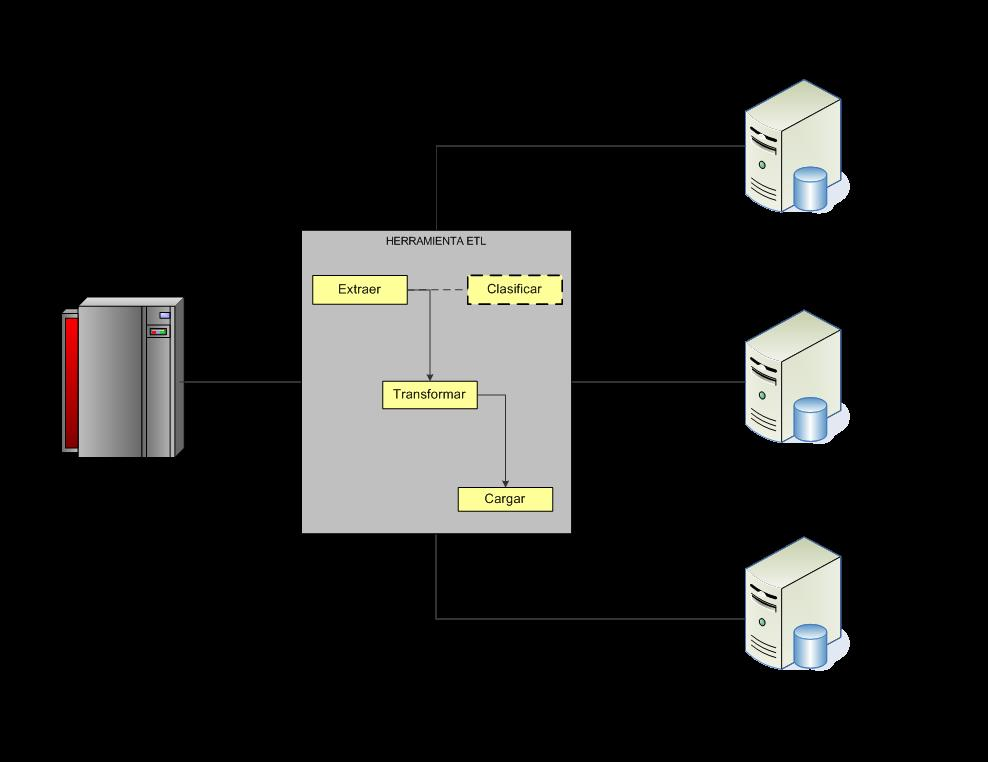
\includegraphics[width=12cm, height=3cm, scale=0.5]{Arquitectura.jpg}
        \caption{Arquitectura de aplicaciones.}
    \label{fig:arquitectura}
  \end{center}
\end{figure}

La arquitectura definida conten\'ia al core bancario como sistema fuente de informaci\'on y enviaba la informaci\'on a la herramienta ETL seleccionada para realizar los procesos de extracci\'on, transformaci\'on, clasificaci\'on y carga hacia los sistemas destino y hacia cada uno de los tipos de datos que necesitaban los equipos y bases de datos destino.


\section{Arquitectura de aplicaciones (Arquitectura detallada)}
La arquitectura dise\~nada se encontraba dividida en cuatro capas y representan el flujo de informaci\'on entre cada una de dichas capas. La capa de interfaz de usuario donde se realizaron todas las tareas de monitoreo, manejo de la herramienta y visualizaci\'on de datos en el sistema destino. La capa de presentaci\'on \'unicamente conten\'ia el servidor de correo que env\'ia la informaci\'on a la capa de interfaz de usuario. Por su parte la capa de integraci\'on conten\'ia los procesos de la herramienta ETL; as\'i como la base de datos stage y la base de datos de cat\'alogos; esta capa tambi\'en inclu\'ia a las aplicaciones que env\'iaban informaci\'on complementaria a los sistemas destino. Finalmente contabamos con la capa de datos que conten\'ia a los sistemas destino, el sistema fuente y al servidor de control de usuarios a trav\'es del directorio activo. La funcionalidad de cada capa as\'i como el flujo de datos se describen a continuaci\'on. 

\subsection{Capa de datos}
La capa de datos conten\'ia diferentes funcionalidades dependiendo del servidor de datos del que estemos hablando. El core bancario ten\'ia la funcionalidad de enviar datos a la herramienta ETL a trav\'es del protocolo TCP\/IP. Por sus parte el directorio activo al manejar informaci\'on de los usuarios de la herramienta ten\'ia la funcionalidad de autenticar a cada usuario que acced\'ia a la herramienta otorg\'andole los permisos necesarioa para ejecutar las tareas dentro de la herramienta ETL, la comunicaci\'on entre la herramienta ETL y el directorio activo se realiz\'o mediante el protocolo LDAP. 

Por su parte los sistemas destino deber\'ian de tener la capacidad de recibir los datos de parte de la herramienta ETL; as\'i como de parte de los ETL's actuales de la instituci\'on financiera y que complementaban la informaci\'on del core bancario; los sistemas destino reciben los datos mediante el protocolo TCP/IP independientemente de la herramienta ETL que los env\'ie.

\subsection{Capa de integraci\'on}
La capa de integraci\'on tiene la funcionalidad de integrar los datos entre las diferentes aplicaciones; la herramienta ETL contiene todos los servicios para la extracci\'on de datos del core bancario, transformarlos y cargarlos en los diferentes sistemas destinode la capa de datos. La herramienta ETL tiene la funcionalidad de enviar los datos a la base de datos stage \footnote{Las bases de datos llamadas stage, son bases de datos temporales o de paso antes de llevar la informaci\'on a su destino final.} así como a la base de datos de cat\'alogos. El proceso deb\'ia enviar v\'ia FTP los archivos de texto a una direcci\'on espec\'ifica dentro de un servidor para que el ETL de lsistema antilavado tome los archivos y complemente la informaci\'on que ser\'a enviada v\'ia TCP/IP a la aplicaci\'on de usuario final. A su vez, el proceso ETL tambi\'en env\'ia informaci\'on a uno de los ETL's del sistema de reportes para que sea complementada por parte del sistema de conciliaci\'on bancaria y sea enviada a la base de datos final de reportes.

\subsection{Capa de presentaci\'on}
LA capa de presentaci\'on de la instituci\'on financiera conten\'ia s\'olamente un servidor de correo; la principal funcionalidad del servidor de correo era proporcionar a los usuarios la informaci\'on de los procesos; es decir, recib\'ia informaci\'on del estatus de los procesos ETL y a su vez enviar\'ia la informaci\'on de este estatus al usuario final.

\subsection{Capa de interfaz de usuario}
La funcionalidad de la capa de interfaz de usuario era administrar la informaci\'on que se recibe del servidor de correo as\'i como de las diferentes aplicciones con las que contaba la instituci\'on financiera. Esta capa era capaz de soportar un ambiente gr\'afico que permit\'ia a los usuarios administrar, construir y dise\~nar sus propios elementos. 

\section{Tecnolog\'ia conceptual}
A continuaci\'on definiremos el dise\~no conceptual de la arquitectura usada para el proyecto, este dise\~no conceptual est\'a dividido en cinco grandes \'areas: Ambiente de desarrollo, herramienta ETL, ambiente de operaci\'on, aplicaciones de la instituci\'on financiera y la capa de infraestructura; de cada una de ellas hablaremos durante este capitulo. 

\begin{figure}[htb]
  \begin{center}
    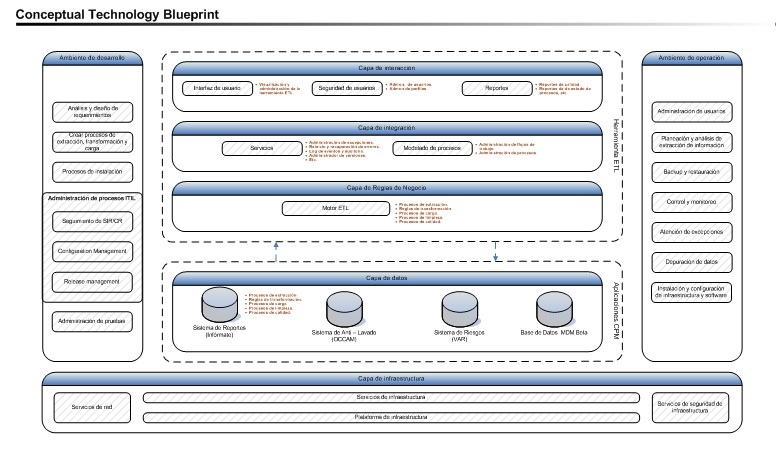
\includegraphics[width=12cm, height=4.5cm, scale=0.5]{Tecnologia_Conceptual.jpg}
        \caption{Tecnolog\'ia conceptual.}
    \label{fig:conceptual}
  \end{center}
\end{figure}

\subsection{Ambiente de desarrollo}
Dentro del ambiente de desarrollo se encuentran definidas todas las actividades que se requieren tener para la construcci\'on de los procesos ETL, as\'i como la administraci\'on de los procesos y las pruebas. El ambiente de desarrollo tiene los siguientes componentes:

\begin{itemize}
\item \textit{An\'alisis y dise\~no de requerimientos}: Dentro de la etapa de an\'alisis y dise\~no de requerimientos encontramos la documentaci\'on de las fuentes y destinos de datos que ser\'an procesadas mediante el ETL; el an\'alisis de requerimientos abarca los requerimientos funcionales y t\'ecnicos que requiere la instituci\'on financiera para poder generar los datos en los sistemas destino. 
Por su parte el dise\~no de los requerimientos incluy\'o el dise\~no funcional y t\'ecnico de todos los procesos a implementar dentro del ETL as\'i como la definici\'on de las reglas de programaci\'on y est\'andares que se ten\'ian que seguir para un mejor desarrollo del proceso.
\item \textit{Creaci\'on de procesos de extracci\'on, transformaci\'on y carga}: Una vez realizado el an\'alisis y dise\~no de los procesos, el siguiente paso es construir los procesos ETL dentro de la herramienta seleccionada; para realizar este desarrollo se deber\'a de basar en el dise\~no funcional, en las reglas de transformaci\'on y en las reglas de negocio definidas dentro del propio dise\~no. El proceso de extracci\'on para la primera iteraci\'on fue solamente del Core Bancario ICBS, mientras que las transformaciones y la carga se realiz\'o de acuerdo al sistema al que se cargaron los datos.
\item \textit{Procesos de instalaci\'on}: Los procesos de instalaci\'on se refieren a los procesos a seguir para instalar el ETL dentro de los diferentes ambientes (desarrollo, pruebas y producci\'on); este proceso también incluy\'o la instalaci\'on de la herramienta de ETL en la que se desarrollaron los procesos.
Parte importante del proceso dentro del ambiente de desarrollo fue la administraci\'on de los procesos de ITIL, como parte de este proceso se ten\'ia el seguimiento de reportes de incidencias (SIR) y controles de cambio (CR), la administraci\'on de configuraciones y la administraci\'on de versiones.
\item \textit{Reporte de incidencias y controles de cambio}: Se llev\'o a cabo un control de incidencias y control de cambios para todos los elementos desarrollados dentro del ETL.

\item \textit{Administraci\'on de configuraciones}. La administraci\'on de configuraciones fue parte importante dentro del ambiente de desarrollo por lo que fue necesario tener un registro de todas las configuraciones que se realizaron dentro de la herramienta.

\item \textit{Administraci\'on de versiones}. Toda herramienta ETL debe tener una administraci\'on de versiones para llevar el control de todos los cambios hechos en el desarrollo.

\item \textit{Administraci\'on de pruebas}: Como todo proyecto de implementaci\'on, fue necesario llevar una administraci\'on de las pruebas; las pruebas que se llevaron a cabo dentro de este proceso fueron: pruebas unitarias, pruebas de integraci\'on, pruebas de performance y pruebas de usuarios
\end{itemize}

\section{Dise\~no de los programas ETL}
Como parte de la herramienta ETL se integraron tres \'areas que ten\'ian relaci\'on con los requerimientos de negocio: la capa de interacci\'on, la capa de integraci\'on y la capa que conte\'ia las reglas de negocio.

\begin{itemize}
\item[*] Capa de interacci\'on. Esta capa se refer\'ia a la interacci\'on que ten\'ian los usuarios con la herramienta ETL; as\'i como la explotaci\'on de todos los elementos de la misma. Las principales funciones que se ejecutaron dentro de esta capa fueron la interfaz de usuario, la administraci\'on de protocolos de seguridad de usuarios y los reportes.
\item[*] Capa de integraci\'on. En esta capa hicimos referencia a todos los servicios y modelado de procesos necesarios para el buen funcionamiento de nuestra herramienta ETL. Los principales procesos que se tomaron en cuenta fueron los siguientes:
\begin{itemize}
\item[*] \textbf{Servicios}. Servicios necesarios para el manejo de errores, excepciones, versiones, as\'i como servicios adicionales necesarios para los procesos de extracci\'on, transformaci\'on y carga. Tales servicios se dividieron en: Administraci\'on de excepciones, reinicio y recuperaci\'on de errores, registros de eventos y auditoria y administraci\'on de versiones.
\item[*] \textbf{Modelado de procesos}. Fueron principalmente los procesos necesarios para la creaci\'on de los programas ETL. 
\end{itemize}
\item[*] Reglas de negocio. Dentro de este proceso definimos las reglas para la transformaci\'on y carga correcta de los datos en la base de datos, as\'i como la funcionalidad correcta que requer\'ia la entidad financiera. La principal herramienta que se tuvo en esta capa, fue el motor ETL y sus principales tareas fueron las siguientes:
\begin{itemize}
\item[*] \textbf{Procesos de extracci\'on.} Definici\'on de todos los procesos utilizados para realizar la extracci\'on de datos
\item[*] \textbf{Reglas de transformaci\'on.} Definici\'on de todas las transformaciones utilizadas desde la extracci\'on de datos hasta la carga de los mismos en la nueva estructura de base de datos.
\item[*] \textbf{Proceso de carga de datos.} DEscripci\'on de los procesos de carga de datos a cada uno de los sistemas destino.
\item[*] \textbf{Proceso de limpieza de datos.} Descripci\'on de los procesos de limpieza de datos como: direcciones, tel\'efonos, nombres, RFCs y fechas.
\item[*] \textbf{Procesos de calidad.} Descripci\'on de los procesos a seguir de acuerdo a los est\'andares de datos para tener una mejor calidad en la informaci\'on. 
\end{itemize}
\end{itemize}

\section{Capa de datos}
La capa de datos estaba conformada por los diferentes sistemas desde donde se extrajo la informaci\'on as\'i como los sistemas donde se almacenar\'ian los datos. Como sistema para extracci\'on de datos solo se consider\'o un sistema, mientras que la carga se realiz\'o hacia tres diferentes sistemas de la instituci\'on financiera. A continuaci\'on describo el tipo de informaci\'on que se procesaba en cada uno de los sistemas destino:
\begin{itemize}
\item[*] Se ten\'ia el sistema de detecci\'on de fraudes o posible mal manejo de una cuenta; esta detecci\'on se realizaba mediante el monitoreo de las cuentas que se enviaban a cada uno de los archivos generados por el procesador principal de transacciones bancarias.
\item[*] El sistema de manejo de riesgos conten\'ia la informaci\'on de las cuentas con pagos vencidos o que presentaban alg\'un grado de morosidad. Esta informaci\'on tambi\'en se obten\'ia del procesador principal de transacciones bancariasy ser\'ia procesada por la herramienta ETL que se implement\'o.
\item[*]Finalmente, exist\'ia el sistema para el manejo de los reportes operativos que requer\'ia la organizaci\'on. La principal tarea de este sistema era generar reportes regulatorios previamente definidos, as\'i como extracci\'on de informaci\'on bajo demanda.
\end{itemize}

\chapter{Dise\~no detallado}
\section{Dependencias y frecuencia de las extracciones de datos}
Como primer paso dentro dle proceos de extracci\'on se identificaron las dependencias de los sistemas origen con otros procesos, tareas o reglas de negocio dentro de la organizci\'on, as\'i como la frecuencia esperada o deseada de la extracci\'on de datos. La extracci\'on de datos se realiz\'o con una periodicidad diaria; esto debido a que al tratarse del sistema principal de la instituci\'on financiera la informaci\'on se actualizaba de manera diaria. La herramienta ETL nos permiti\'o identificar aquellas tablas y campos que sufrian modificaciones, de tal forma que se extrajo solo la informaci\'on que sufr\'ia cambios a lo largo del d\'ia. La extracci\'on de datos se realiz\'o en un horario no operativo, a fin de no afectar la operaci\'on de la instituci\'on; adem\'as este proceso depend\'ia del termino del proceso de cierre diario de operaciones. Solamente uan vez que el proceso hubiera terminado comenzaba la extracci\'on por parte de la herramienta ETL; este proceso contaba con una ventana de procesamiento de 5 horas. La extracci''on fue almacenada en la base de datos temporal dentro de la herramienta ETL.
\subsection{Extracci\'on inicial}
En la extracci\'on inicial se realizaron las siguientes transformaciones:
\begin{itemize}
\item[*] Transformaci\'on de fecha jualiana a fecha gregoriana.
\item[*] Cambio en los tipos de dato al momento de almacenarlos en la tabla temporal; principalmente transformaci\'on del tipo de dato \textit{char} al tipo de dato \textit{varchar} y los datos n\'umericos a decimal.
\end{itemize}
Al momento de que se terminaba la extracci\'on de datos, se cerraba la conexi\'on a la base de datos del procesador principal de transacciones bancarias a fin de liberar la carga de trabajo del mismo para continuar con su operaci\'on diaria. 
\subsection{Extracciones subsecuentes}
Despu\'es de realizada la extracci\'on inicial desde el sistema fuente y con los datos almacenados en el repositorio temporal, las siguientes extracciones se realizaron mediante extracciones incrementales con base en la adici\'on, actualizaci\'on o eliminaci\'on de datos de las tablas seleccionadas. Se consider\'o realizar la extracci\'on total de los registros solo en caso de que las modificaciones o actualizaciones en la base de datos fueran muchas; las condiciones para realizar la extracci\'oncompleta fueron las siguientes:
\begin{enumerate}
\item Exist\'ian cambios en m\'as del 50\% de los registros.
\item Los registros extra\'idos no se encontraban actualizados o conten\'ian errores.
\item Los registros extra\'idos no cuentan con la calidad necesaria.
\end{enumerate}
\subsection{Relaci\'on entre las entidades de datos}
En el siguiente diagrama se puede visualizar la relaci\'on entre las diferentes entidades y los datos que comparten cada uno de ellos.
\begin{figure}[htb]
  \begin{center}
    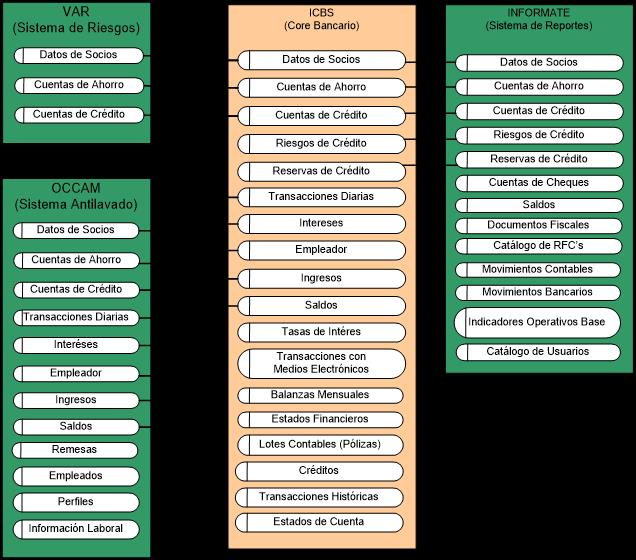
\includegraphics[width=12cm, height=3cm, scale=0.5]{Relacion_entidades.jpg}
        \caption{Datos relacionados en las entidades.}
    \label{fig:arquitectura}
  \end{center}
\end{figure}

En la imagen podemos observar que los diferentes sistemas manejan el mismo tipo de informaci\'on; socios, cuentas, cr\'editos y saldos.

\section{Dise\~no para la transformaci\'on de datos}
La transformaci\'on de los datos ten\'ia varios procesos que se deber\'ian seguir, entre los cuales se encuentra la limpieza de datos, los est\'andares y procedimientos utilizados, as\'i como las reglas de transformaci\'on definidas para cada uno de los sistemas destino. La transformaci\'on de los datos se realiz\'o dentro de la misma base de datos de paso y se almacen\'o en otra instancia de esta misma base de datos. El siguiente diagrama muestra como se realizar\'on las transformaciones requeridas.

\begin{figure}[htb]
  \begin{center}
    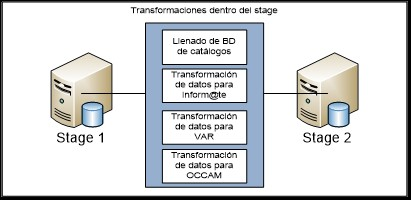
\includegraphics[width=12cm, height=3cm, scale=0.5]{Transformaciones_stage.jpg}
        \caption{Transformaciones en base de datos temporal.}
    \label{fig:arquitectura}
  \end{center}
\end{figure}

A continuaci\'on se detallan las reglas utilizadas para realizar la transfocmac\'on de datos.
\subsection{Limpieza de la fuente de datos}
La limpieza de la fuente de datos \textbf{NO} estaba dentro del alcance del proyecto; sin embargo se realizaron las transformaciones de la fuente de datos para realizar la limpieza de datos hacia los sistemas destino. Como parte de un proceso de calidad de la informaci\'on y limpieza de datos se definier\'on los siguientes criterios: 

\begin{enumerate}
\item Los nombres de los socios deb\'ian contener solamente caracteres alfab\'eticos; no se permitieron caracteres especiales como los siguientes: a"\.","\".","\#","\$", "\%", "\&".
\item Los n\'umeros telef\'onicos deb\'ian contener solamente caracteres num\'ericos y deb\'ian ser de 10 posisciones para tel\'efonos fijos y 13 posiciones para tel\'efonos celulares.
\begin{itemize}
\item[a.] Si \textit{Tipo\_Telefono}  $=$ Casa y Longitud $($Telefono$)$  $=$10 Entonces Telefono\_Casa SiNo Error
\item[b.] Si \textit{Celular} $=$ Casa y Longitud $($Telefono$)$ $=$ 13 Entonces Telefono\_Celular SiNo Error
\end{itemize}  
\item El RFC de los socios deber\'ia ser de 10 o 13 posiciones para las personas f\'isicas y 12 posiciones para las personas morales. En caso de no contar con un RFC valido, el registro era rechazado y enviado a una tabla de auditoria para su correcci\'on dentro del sistema fuente de parte del \'area de tecnolog\'ia de la compa\~nia. 
\item Todos los c\'odigos postales deb\'ian ser de cinco d\'igitos, en caso de existir alg\'un registro con mayor o menor n\'umero, estos deb\'ian de ser enviados a una tabla de auditoria para su correcci\'on dentro del sistema fuente. Se consider\'o una homologaci\'on de datos para los c\'odigos de ciudades y estados. Todos los c\'odigos de estados se homologaron a tres d\'igitos que corresponden a las tres primeras letras de cada estado; se realiz\'o unaexcepci\'on para el caso de Chiapas \(CHS\) que podr\'ia confundirse con Chihuahua \(CHI\).
\item Las fechas se homologaron al formato yyyymmdd y no deb\'ian permitir valores nulos o fechas inv\'alidas.
\end{enumerate}
\subsection{Est\'andares y procedimientos utilizados para la interrelaci\'on de los datos}
Para realizar una estandarizaci\'on de los datos se cre\'o una base de datos temporal que contern\'ia la informaci\'on de todos los campos con los mismos datos pero que su sistema origen era diferente. La creaci\'on de esta tabla temporal fue crear la base para generar una tabla de referencias cruzadas que representara un gobierno de datos o MDM (Master Data Management) por sus siglas en Inglés

\subsection{Reglas utilizadas para la transformaci\'on de datos}
Como regla general para todos los procesos de extracci\'on se realizaron las siguientes transformaciones. 
\begin{itemize}
\item[*] Transformaci\'on de fechas julianas a fechas gregorianas en formato yyyy$/$mm$/$dd.
\item[*] Transformaci\'on de los tipos de dato origen a los tipos de la base de datos stage generada en SQL Server.
\end{itemize}

Los procesos de transformaci\'on para cada destino fueron diferentes debido a las caracter\'isticas de cada uno de los archivos de salida. Dichas transformaciones se realizaron tomando como principal fuente de datos, la base de datos temporal. 

\subsubsection{Sistema de reportes}
\begin{itemize}
\item[-] Todos los campos de fecha que tengan un sufijo \_d deber\'ian de ser convertidas a formato de fecha $($yyyymmdd$)$ para todas las tablas de este sistema. Se pobl\'o la fecha de vencimiento \_D, tomando como base el campo fecha de vencimiento de la tabla de facturaci\'on. La regla de transformaci\'on que se defini\'o fue la siguiente:
\begin{verbatim}
FEC_VENCIMIENTO_5_D = CAST(RIGHT(LTRIM(RTRIM(FEC_VENCIMIENTO_5)),2) +
	LEFT(RIGHT(LTRIM(RTRIM(FEC_VENCIMIENTO_5)),4), 2) +  
	REPLICATE('0', 2-len(LEFT(LTRIM(RTRIM(FEC_VENCIMIENTO_5)), 
	ABS(4-len(LTRIM(RTRIM(FEC_VENCIMIENTO_5))))))) +
	LEFT(LTRIM(RTRIM(FEC_VENCIMIENTO_5)), 
	ABS(4-len(LTRIM(RTRIM(FEC_VENCIMIENTO_5))))) AS DATETIME)     
	WHERE  FEC_VENCIMIENTO_5 > 0
\end{verbatim}
\item[-] Para el campo Fecha de último saldo se tom\'o la fecha de vencimiento m\'as antigua que se ten\'ia.
\item[-] Para obtener el n\'umero de cr\'editos de un socio se realiz\'o la siguiente regla.
\begin{verbatim}
	NO_CREDITOS =  NO_CREDITOS 
	WHERE  NO_SOCIO IN NO_SOCIO de la tabla CIF_CREDITOS.
	Si NO_CREDITOS = NULL Entonces NO_CREDITOS = 0
\end{verbatim} 
\item[-] La descripci\'on de la informaci\'on correspondiente a las garant\'ias deb\'ia de estar vacio en la tabla destino.
\item[-] Para almacenar la fecha de \'ultimo monto con saldo se tom\'o la fecha de vencimiento m\'as antigua que se ten\'ia para cada registro dentro de la tabla de saldos \textit{LN\_SALDOS.}
\item[-] Se realiz\'o una validaci\'on sobre el tipo de cuenta para confirmar su valor $=$ 1 $($Personas f\'isicas$)$ o 6; en estos casos se coloc\'o un valor 20 dentro del campo Tipo\_producto de la tabla TA\_SALDOS.
\item[-] El n\'umero de docio para poblar la tabla TA\_SALDOS se obtuvo de la tabla de cuentas por socio, pero solamente de aquellas cuentas cuyo tipo de producto era 4 u 8 y que tuvieran un saldo en la tabla TA\_SALDOS.
\item[-] Se calcul\'o el n\'umero de cr\'editos de cada socio y este valor se grab\'o en la tabla CIF\_INFGEN; en caso de que el n\'umero de cr\'editos fuera nulo se coloc\'o un valor por default 0.
\item Se insert\'o el n\'umero de socio dentro de la tabla TA\_CTAXSOCIO para aquellos n\'umeros de cuenta menores a 20000000000 y cuya clave de relaci\'on fuera 'SOW' u 'OWN'. El n\'umero de socio eran los 10 d\'igitos de la derecha de cada n\'umero de cuenta.
\item[-] Se defini\'o que para el campo descripci\'on perteneciente a la tabla LN\_GARANTIAS deber\'ia poblarse con un valor NULL a pesar de tener mapeado un campo del cu\'al se extra\'ia la informaci\'on. 
\item[-] El campo Periodo de la tabla LN\_SALDOS se asign\'o con un valor fijo = 'M'.
\item[-] El campo frecuencia de la tabla LN\_SALDOS se asign\'o con un valor fijo $=$ 30. 
\end{itemize}
La regla de transformaci\'on que se utiliz\'o durante la extracci´\'on 
\subsubsection{Reglas para el sistema para prevenci\'on de lavado de dinero}
Las reglas definidas para este sistema son las siguientes:
\begin{itemize}
\item[-] Se definieron algunos valores est\'aticos para los tres primeros campos de cada uno de los archivos generados; estos valores son los siguientes:
\begin{enumerate}
\item Valor fijo 'CMPS' para el primer campo.
\item Valor fijo 'T' para el segundo campo.
\item Valor fijo 'F' para el tercer campo.
\end{enumerate}
\item[-] Para la generaci\'on del archivo de cuentas se tomaron solo aquellas cuentas que tuvieron movimientos durante el d\'ia.
\item[-] Solamente se tomaron en cuenta los siguientes tipos de cuenta: Parte social, cuenta mexicana, servicuenta y cuentamiga.
\item[-] Si el tipo CIF es una persona moral (CUTYP $=$ 5), entonces el campo CompanyLegalId se pobl\'o con dicho valor, en caso contrario se asign\'o un valor constante vacio " ".
 
\end{itemize}

\section{Arquitectura aplicativa}

\section{Arquitectura de negocio}
\section{Arquitectura de datos}
Como se explic\'o en los capitulos anteriores, la instituci\'on financiera contaba con diferentes procesos ETL que extra\'ian informaci\'on del sistema principal. Estos sistemas trabajaban de manera independiente por lo que cada sistema destino ten\'ia su base de datos temporal antes de enviarla a su destino. La arquitectura se encuentra detallada en el siguiente diagrama:

\begin{figure}[htb]
  \begin{center}
    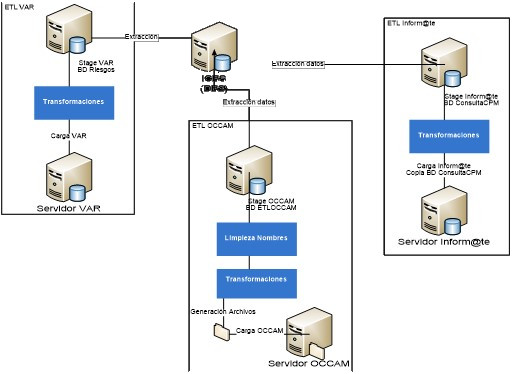
\includegraphics[width=12cm, height=3cm, scale=0.5]{Arquitecturadatos_actual.jpg}
        \caption{Arquitectura de datos actual.}
    \label{fig:arquitecturaactual}
  \end{center}
\end{figure}

Como se observa en la imagen anterior, exist\'ian muchas bases de datos intermedias entre la fuente de datos y los sistemas destino; la arquitectura definida dentro de este proyecto, nos permite tener una sola base de datos temporal, as\'i como una sola capa de integraci\'on de datos. El siguiente diagrama muestra el dise\~no de la arquitectura desarrollada: 

\begin{figure}[htb]
  \begin{center}
    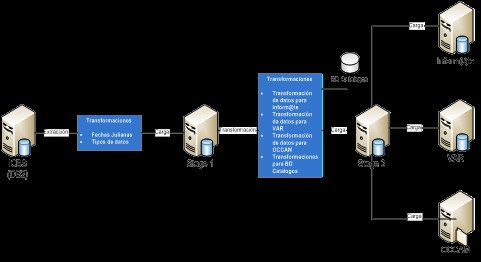
\includegraphics[width=12cm, height=3cm, scale=0.5]{Arquitectura_final.jpg}
        \caption{Arquitectura de datos actual.}
    \label{fig:Arquitecturafinal}
  \end{center}
\end{figure}
Arquitectura_final

\section{Arquitectura de infraestructura}

 "Diseño de arquitectura aplicativa", "Arquitectura de negocio", "Arquitectura de datos" y "Arquitectura de infraestructura"

\chapter*{Modelo de datos} \label{cap.modelo}% si no queremos que a�ada la palabra "Capitulo"
\addcontentsline{toc}{section}{Modelo de datos} % si queremos que aparezca en el �ndice
\markboth{Modelo de datos}{Modelo de datos} % encabezado

5.1. Modelo de datos l�gico

5.2. Modelo de datos f�sico

\chapter*{Est\'andares de programaci\'on} \label{cap.estandares}% si no queremos que a�ada la palabra "Capitulo"
\addcontentsline{toc}{section}{Est\'andares de programaci\'on} % si queremos que aparezca en el �ndice
\markboth{Est\'andares de programaci\'on}{Est\'andares de programaci\'on} % encabezado

dalsdkla

\chapter*{Conclusiones} \label{cap.conclusiones}% si no queremos que a�ada la palabra "Capitulo"
\addcontentsline{toc}{section}{Conclusiones} % si queremos que aparezca en el �ndice
\markboth{Conclusiones}{Conclusiones} % encabezado


\end{document}
